% ============================================================
%  Chapter 12: Delivering Parcels
%  Nature Inspired Optimisation for Delivery Problems (2022)
%  Self-contained Beamer lecture slides
% ============================================================
\documentclass[aspectratio=169,10pt]{beamer}

\usetheme{Madrid}
\usecolortheme{seahorse}

\usepackage{amsmath,amssymb}
\usepackage{graphicx}
\usepackage{booktabs}
\usepackage{array}
\usepackage{xcolor}
\usepackage{listings}
\usepackage{tikz}
\usepackage{pgfplots}
\pgfplotsset{compat=1.18}
\usetikzlibrary{shapes.geometric, arrows.meta, positioning, fit, calc}
\usepackage{microtype}
\usepackage{hyperref}
\usepackage{caption}

\graphicspath{{figures/}}

% ------ listings style ------
\lstset{
  language=Python,
  basicstyle=\ttfamily\scriptsize,
  numbers=left,
  numberstyle=\tiny\color{gray},
  frame=single,
  backgroundcolor=\color{gray!7},
  commentstyle=\color{green!50!black}\itshape,
  keywordstyle=\color{blue!70!black}\bfseries,
  stringstyle=\color{orange!80!black},
  breaklines=true,
  showstringspaces=false,
  tabsize=4,
  xleftmargin=1.5em,
  framexleftmargin=1.5em,
}

\setbeamertemplate{footline}[frame number]
\setbeamertemplate{navigation symbols}{}

% ------ title info ------
\title[Ch.12: Delivering Parcels]{Chapter 12: Delivering Parcels}
\subtitle{Nature Inspired Optimisation for Delivery Problems (2022)}
\author{Based on Urquhart, H\"{o}hl, Hart (2019, 2021)}
\date{}

% ============================================================
\begin{document}

\begin{frame}
  \titlepage
\end{frame}

% ────────────────────────────────────────────────
\begin{frame}[allowframebreaks]{Chapter Overview}

This chapter investigates the \textbf{Micro-Depot Vehicle Routing Problem (MDVRP)}
applied to parcel delivery in urban city centres.
The core challenge is real and urgent: as online shopping has grown dramatically,
freight vehicles are causing serious traffic congestion and harmful emissions
in city centres.
The chapter proposes a nature-inspired solution that illuminates the full space
of possible delivery strategies rather than finding a single ``best'' answer.

\medskip

The chapter is structured around five main topics:

\begin{enumerate}
  \item \textbf{Problem Description} --- what micro-depots are, why they help,
        and how the Edinburgh parcel-delivery scenario is formulated.
  \item \textbf{Methodology} --- the MAP-Elites illumination algorithm
        combined with a flexible genetic representation.
  \item \textbf{Implementation} --- the software architecture, chromosome encoding,
        and decoding procedure (with Algorithm~24).
  \item \textbf{Results} --- parallel coordinates visualisation, heatmaps,
        and FlexGP-extracted human-readable policies.
  \item \textbf{Conclusions} --- key insights about when and how to use
        micro-depots effectively.
\end{enumerate}

\medskip

\begin{alertblock}{Key Insight}
  Rather than asking ``What is the single best delivery plan?'',
  MAP-Elites asks ``What is the best delivery plan \emph{for each type of situation}?''
  This produces an entire library of solutions that a logistics planner
  can explore.
\end{alertblock}

\end{frame}

% ============================================================
\section{12.1 Problem Description}
% ============================================================

\begin{frame}[allowframebreaks]{12.1 The Urban Delivery Problem}

Urban last-mile delivery faces a fundamental conflict:
customers want fast, reliable delivery of parcels,
but dense cities cannot absorb unlimited freight-vehicle traffic.
The resulting congestion harms everyone --- it slows all vehicles,
raises fuel consumption, and increases emissions of \(\text{CO}_2\)
and fine particles.

\medskip

\begin{block}{What is a Micro-Depot (MD)?}
  A \textbf{micro-depot} (sometimes called a \emph{city consolidation centre})
  is a small, strategically placed storage point within or near a city centre.
  A large supply vehicle --- which need not enter the congested core ---
  restocks each micro-depot once or a few times per day.
  From the micro-depot, small and low-emission couriers (walkers, cyclists,
  electric vehicles) make the final deliveries to individual addresses.
  This two-tier approach keeps large vehicles on arterial roads
  and puts clean, nimble couriers on narrow city streets.
\end{block}

\medskip

Three categories of cost or impact are of interest to city planners:

\begin{itemize}
  \item \textbf{Traffic congestion} --- how many vehicle trips enter the city core.
  \item \textbf{Emissions} --- total \(\text{CO}_2\)-equivalent produced.
  \item \textbf{Delivery time} --- how long customers wait.
\end{itemize}

These three objectives often conflict with each other, motivating the
multi-characteristic illumination approach.

\end{frame}

% ────────────────────────────────────────────────
\begin{frame}[allowframebreaks]{12.1 The Edinburgh Scenario}

The chapter uses a \textbf{real-world data scenario based on Edinburgh, Scotland}.
The city centre has a historic layout with narrow streets and restricted
access zones, making it a natural testbed for micro-depot strategies.

\medskip

\begin{columns}[T]
  \begin{column}{0.55\textwidth}
    \begin{block}{Problem Data}
      \begin{itemize}
        \item A set of delivery addresses (customers) located within
              the Edinburgh city centre area.
        \item A main depot located outside the city centre
              (labelled \emph{D0}).
        \item Several candidate micro-depot locations
              distributed across the city, each identified
              by a unique ID (MD1, MD2, \ldots).
        \item A supply vehicle that can visit any micro-depot
              to drop off parcels.
        \item Three courier types operating from micro-depots:
              \textbf{walking}, \textbf{cycling},
              and \textbf{electric van (EV)}.
      \end{itemize}
    \end{block}
  \end{column}
  \begin{column}{0.42\textwidth}
    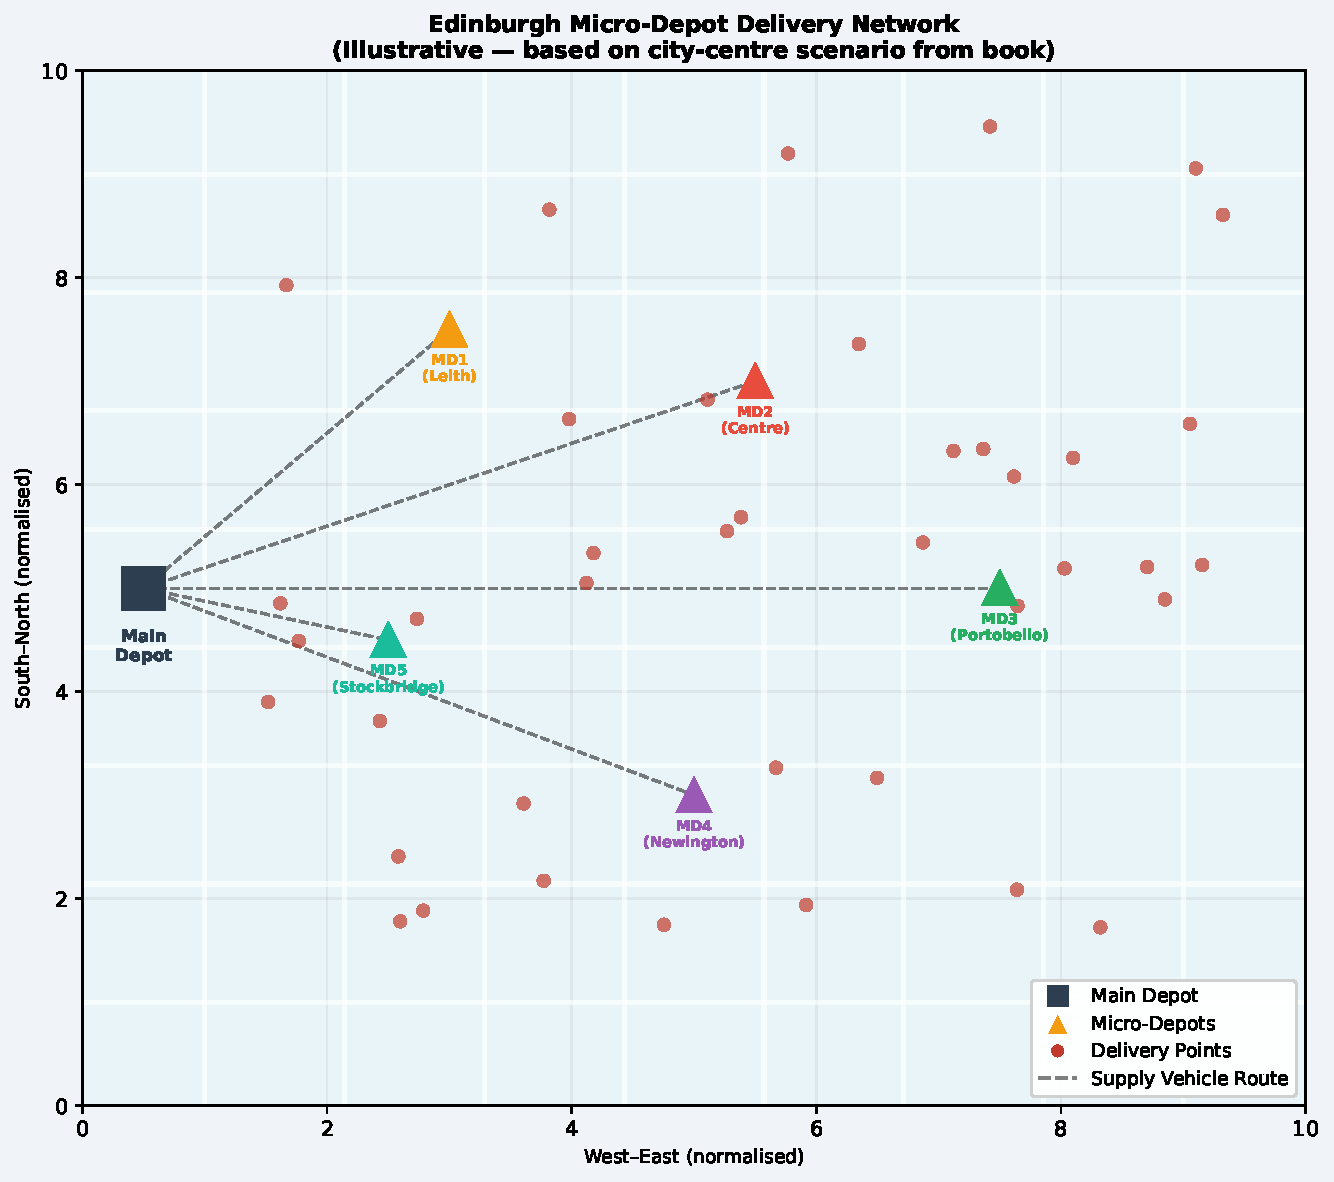
\includegraphics[width=\linewidth]{fig_edinburgh_network}
    \captionof*{figure}{\scriptsize Illustrative Edinburgh delivery network.
      Square = main depot; triangles = micro-depots;
      dots = customer delivery points.}
  \end{column}
\end{columns}

\medskip

The problem is defined over \textbf{10 separate problem instances},
each representing, for example, one day's worth of deliveries
(a subset of the full customer set).
Each instance is treated as an independent optimisation run,
and results are aggregated to see patterns across instances.

\end{frame}

% ────────────────────────────────────────────────
\begin{frame}[allowframebreaks]{12.1 Courier Types and Their Trade-offs}

The three courier types differ in speed, capacity, and environmental impact.
Understanding these differences is essential for interpreting the results.

\medskip

\begin{block}{Courier Type Comparison}
  \begin{tabular}{lllll}
    \toprule
    \textbf{Type} & \textbf{Speed} & \textbf{Capacity} & \textbf{Emissions} & \textbf{Network access} \\
    \midrule
    Walking & Very slow & Very low & Zero & All paths \\
    Cycling & Slow & Low & Zero & Cycle paths + roads \\
    Electric Van (EV) & Moderate & High & Very low & Roads only \\
    Supply Vehicle & Fast & Very high & Moderate--High & Arterial roads \\
    \bottomrule
  \end{tabular}
\end{block}

\medskip

Paths available to couriers depend on vehicle type.
Walking and cycling couriers can use pedestrian paths and cycle lanes
that are not accessible to electric vans or the supply vehicle.
The routing algorithm (nearest-neighbour heuristic) must respect
these path restrictions when computing distances.

\medskip

\begin{alertblock}{Key Insight}
  Electric vans are fast enough to cover more deliveries per time unit
  and carry more parcels, but they are restricted to road networks.
  Cyclists and walkers are slower but can reach destinations
  that road vehicles cannot, and they produce zero emissions.
  The optimal policy depends on the ratio of narrow-street
  deliveries to road-accessible deliveries.
\end{alertblock}

\end{frame}

% ────────────────────────────────────────────────
\begin{frame}[allowframebreaks]{12.1 Solution Characteristics: Measuring the Archive}

Rather than tracking a single objective value, MAP-Elites characterises
each solution by \textbf{seven behavioural dimensions}.
These dimensions describe \emph{how} a solution achieves its deliveries,
not merely whether it is feasible.

\medskip

\begin{block}{The Seven Solution Characteristics (Table 12.1)}
  \begin{tabular}{lll}
    \toprule
    \textbf{Label} & \textbf{Description} & \textbf{Scale} \\
    \midrule
    $X_1$ & Number of micro-depots used & 1--10 \\
    $X_2$ & Percentage of deliveries routed via micro-depots & 1--10 \\
    $X_3$ & Number of cycling couriers used & 1--10 \\
    $X_4$ & Number of walking couriers used & 1--10 \\
    $X_5$ & Number of EV couriers used & 1--10 \\
    $X_6$ & Total delivery time (normalised) & 1--10 \\
    $X_7$ & Total emissions (normalised) & 1--10 \\
    \bottomrule
  \end{tabular}
\end{block}

\medskip

Each characteristic is \textbf{normalised to the integer range 1--10},
which means the archive has at most $10^7 = 10{,}000{,}000$ cells.
In practice, only a fraction of cells are occupied, because many
combinations of characteristics are infeasible or never discovered.

\medskip

\begin{block}{Label Mapping (Table 12.2)}
  To make policies human-readable, the integer scale is translated
  into natural-language labels:
  \begin{tabular}{ll}
    \toprule
    \textbf{Range} & \textbf{Label} \\
    \midrule
    1--2 & Very Low \\
    3--4 & Low \\
    5--6 & Medium \\
    7--8 & High \\
    9--10 & Very High \\
    \bottomrule
  \end{tabular}
\end{block}

\medskip

For example, a solution with $X_5 = 9$ would be labelled
``EVs Used = Very High''.
This label system is used by FlexGP (Section~12.2) to produce
human-readable policy statements.

\medskip

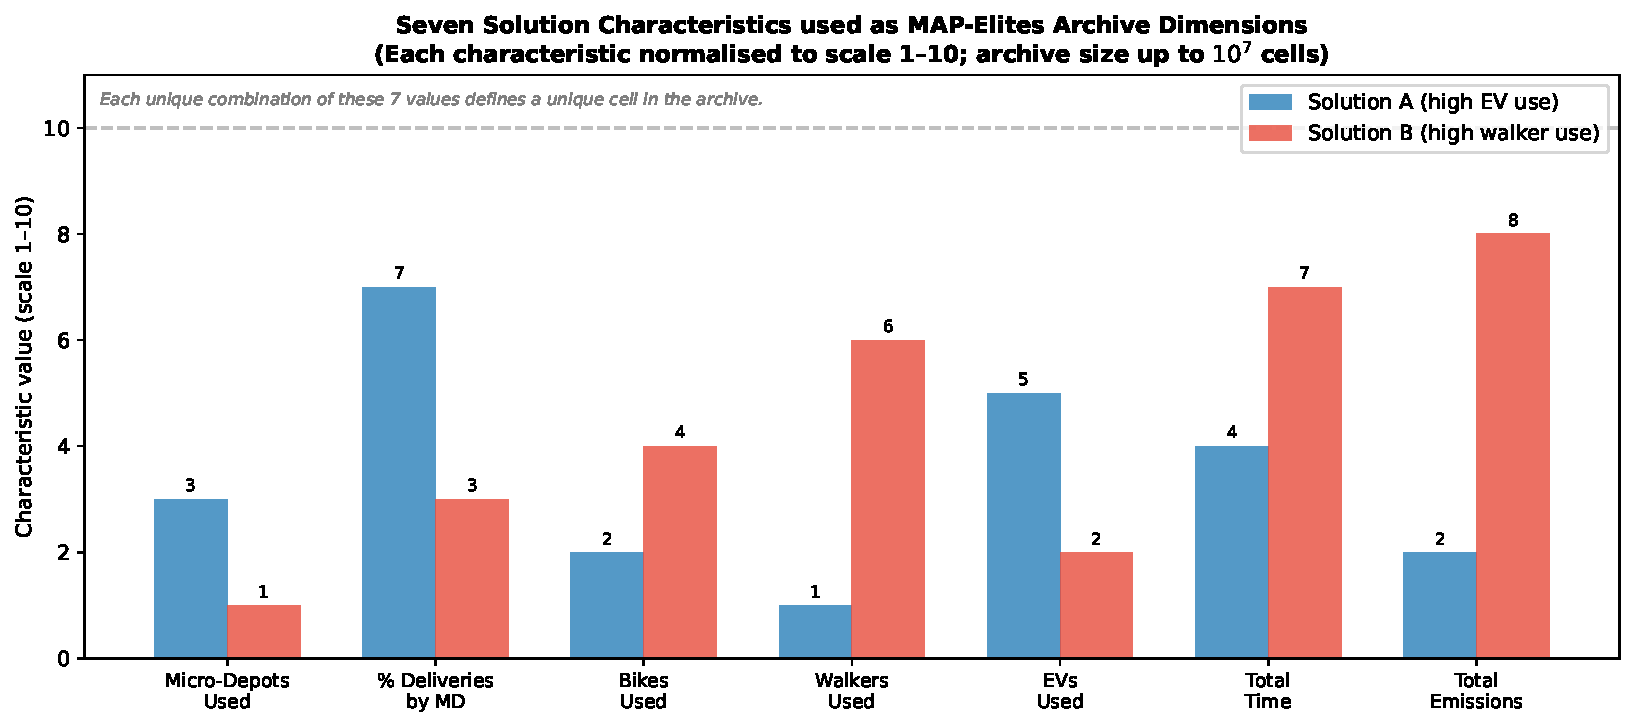
\includegraphics[width=0.85\textwidth]{fig_solution_characteristics}
\captionof*{figure}{\scriptsize Two contrasting solutions across the seven
  characteristic dimensions. Solution A maximises EV use and achieves
  low emissions; Solution B relies on walking couriers and suffers
  higher time and emissions.}

\end{frame}

% ============================================================
\section{12.2 Methodology}
% ============================================================

\begin{frame}[allowframebreaks]{12.2 Overview of the Hybrid Approach}

The methodology combines three well-established techniques
into a coherent pipeline:

\medskip

\begin{enumerate}
  \item \textbf{MAP-Elites} (from Chapter~5 / Chapter~6 of the book) ---
        an illumination algorithm that fills a multidimensional
        behavioural archive with high-quality solutions.
        Each cell of the archive stores the best solution found
        so far for that particular combination of characteristics.

  \item \textbf{Evolutionary operators} ---
        mutation and crossover on a chromosome-based representation
        generate new candidate solutions for MAP-Elites to evaluate.

  \item \textbf{FlexGP} ---
        a machine-learning rule-extraction tool that reads the
        populated archive and outputs Boolean decision rules
        (policies) that explain which regions of the solution space
        yield good outcomes.
\end{enumerate}

\medskip

\begin{alertblock}{Why this pipeline?}
  A standard genetic algorithm would return a single solution.
  MAP-Elites returns a \emph{library} of solutions, each optimised
  for a different operating scenario.
  FlexGP then converts this library into plain-English policies
  that a manager --- not just an algorithm expert --- can act on.
\end{alertblock}

\end{frame}

% ────────────────────────────────────────────────
\begin{frame}[allowframebreaks]{12.2 MAP-Elites: Illumination Algorithm}

MAP-Elites was introduced by Mouret and Clune (2015) as a way to
\emph{illuminate the solution space} rather than converge to a single point.
The name stands for \textbf{Map of Elites}: it builds a map
(the archive grid) in which each cell holds the best (\emph{elite})
solution found for that cell's combination of characteristics.

\medskip

\begin{block}{MAP-Elites Algorithm (High Level)}
  \begin{enumerate}
    \item \textbf{Initialise}: Generate a random population of solutions.
          For each, evaluate its fitness and compute its $d$-dimensional
          characteristic vector (here $d = 7$).
          Insert each solution into the archive if its cell is empty
          or if it improves on the existing occupant.
    \item \textbf{Repeat} for $N$ iterations:
      \begin{enumerate}
        \item Select a random solution $\mathbf{x}$ from the archive.
        \item Create a new candidate $\mathbf{x}'$ by mutating
              (and optionally crossing over) $\mathbf{x}$.
        \item Evaluate $\mathbf{x}'$: compute its fitness
              and characteristic vector.
        \item Attempt to insert $\mathbf{x}'$ into the archive:
              if its cell is empty, or if it has higher fitness
              than the current occupant, replace the occupant.
      \end{enumerate}
    \item \textbf{Output}: the entire archive --- a map of the best
          solution found for each region of behaviour-space.
  \end{enumerate}
\end{block}

\medskip

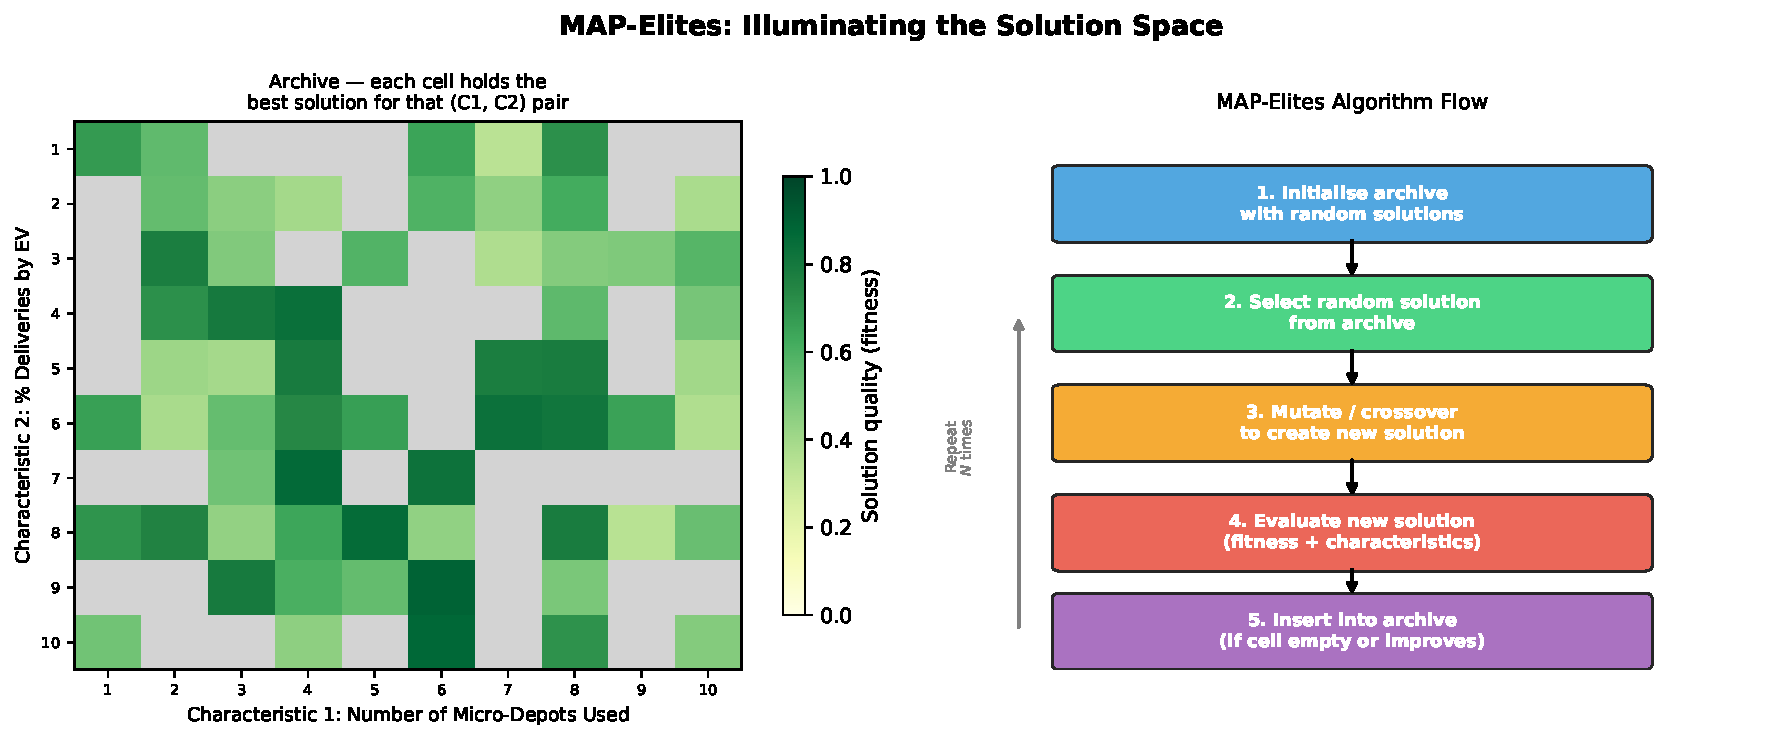
\includegraphics[width=0.9\textwidth]{fig_map_elites_archive}
\captionof*{figure}{\scriptsize Left: example 2D archive slice showing solution
  quality (greener = better) across two characteristics.
  Right: the five-step MAP-Elites algorithm loop.}

\end{frame}

% ────────────────────────────────────────────────
\begin{frame}[allowframebreaks]{12.2 Use of Machine Learning: FlexGP}

After MAP-Elites produces an archive of solutions, the chapter
uses \textbf{FlexGP} (Flexible Genetic Programming) to extract
human-interpretable policies from the archive data.

\medskip

FlexGP is a machine-learning classifier that learns Boolean expression trees.
The archive is converted into a supervised learning dataset:
each solution in the archive becomes one training example.
The input features are the seven solution characteristics ($X_1,\ldots,X_7$),
and the output label is a binary classification (0 or 1) derived from
the solution's performance on the objective of interest (e.g.\ emissions).

\medskip

\begin{block}{Training Data Format}
  Each row of the training data looks like:
  \[
    (X_1,\; X_2,\; X_3,\; X_4,\; X_5,\; X_6,\; X_7,\; \text{label})
  \]
  where the label is 1 if the solution has ``very low emissions''
  and 0 if it has higher emissions.
  An example data fragment from the book:
\begin{center}\ttfamily\scriptsize
  4,2,10,6,8,7,1 \\
  6,5,5,6,10,2,0 \\
  7,1,10,3,2,1,1 \\
  \ldots
\end{center}
  Here column~7 (the last) is the label: 1 = very low emissions, 0 = higher.
\end{block}

\medskip

FlexGP's task is to find a compact Boolean rule (a short decision tree
expressed as a logical formula) that correctly classifies as many
training examples as possible.
The result is a policy that a logistics manager can read, understand,
and apply to new situations without needing to re-run the algorithm.

\end{frame}

% ────────────────────────────────────────────────
\begin{frame}[allowframebreaks]{12.2 FlexGP Policy: Structure and Interpretation}

FlexGP evolves Boolean condition trees using the seven characteristic
variables.
Each interior node is AND or OR; each leaf is a range condition
on one variable.
The tree is then translated into natural language using
the label table (Table~12.2).

\medskip

\begin{block}{Example FlexGP Policy (Low Emissions)}
  The raw policy extracted from the archive is:
  \[
    \bigl((1.0 \le X_5 \le 8.6\ \mathbf{and}\ 1.0 \le X_4 \le 2.0)\
    \mathbf{and}\ (1.0 \le X_2 \le 8.4\ \mathbf{or}\ 1.0 \le X_3 \le 2.7)\bigr)
  \]
  where:
  \begin{itemize}
    \item $X_2$ = percentage of deliveries via micro-depots,
    \item $X_3$ = number of bicycles (bikes) used,
    \item $X_4$ = number of walking couriers used,
    \item $X_5$ = number of electric vehicles (EVs) used.
  \end{itemize}
\end{block}

\medskip

Substituting the label names, the policy becomes:
\[
  ((EVs\text{Used} \le \text{VeryHigh}\ \mathbf{and}\
    \text{WalkersUsed} \le \text{VeryLow})\
  \mathbf{and}\
  (\%\text{ByMD} \le \text{High}\ \mathbf{or}\
   \text{BikesUsed} \le \text{Low}))
\]

\begin{alertblock}{Plain-English Interpretation}
  \textit{``Maximise the use of EVs, make minimal use of walking couriers,
  and either send a large fraction of deliveries through micro-depots
  or minimise the use of bicycles.''}
  This makes intuitive sense: EVs are the cleanest powered couriers,
  walkers are slow and cover few deliveries per hour, and MDs
  allow more goods to be dispatched concurrently from distributed
  points.
\end{alertblock}

\medskip

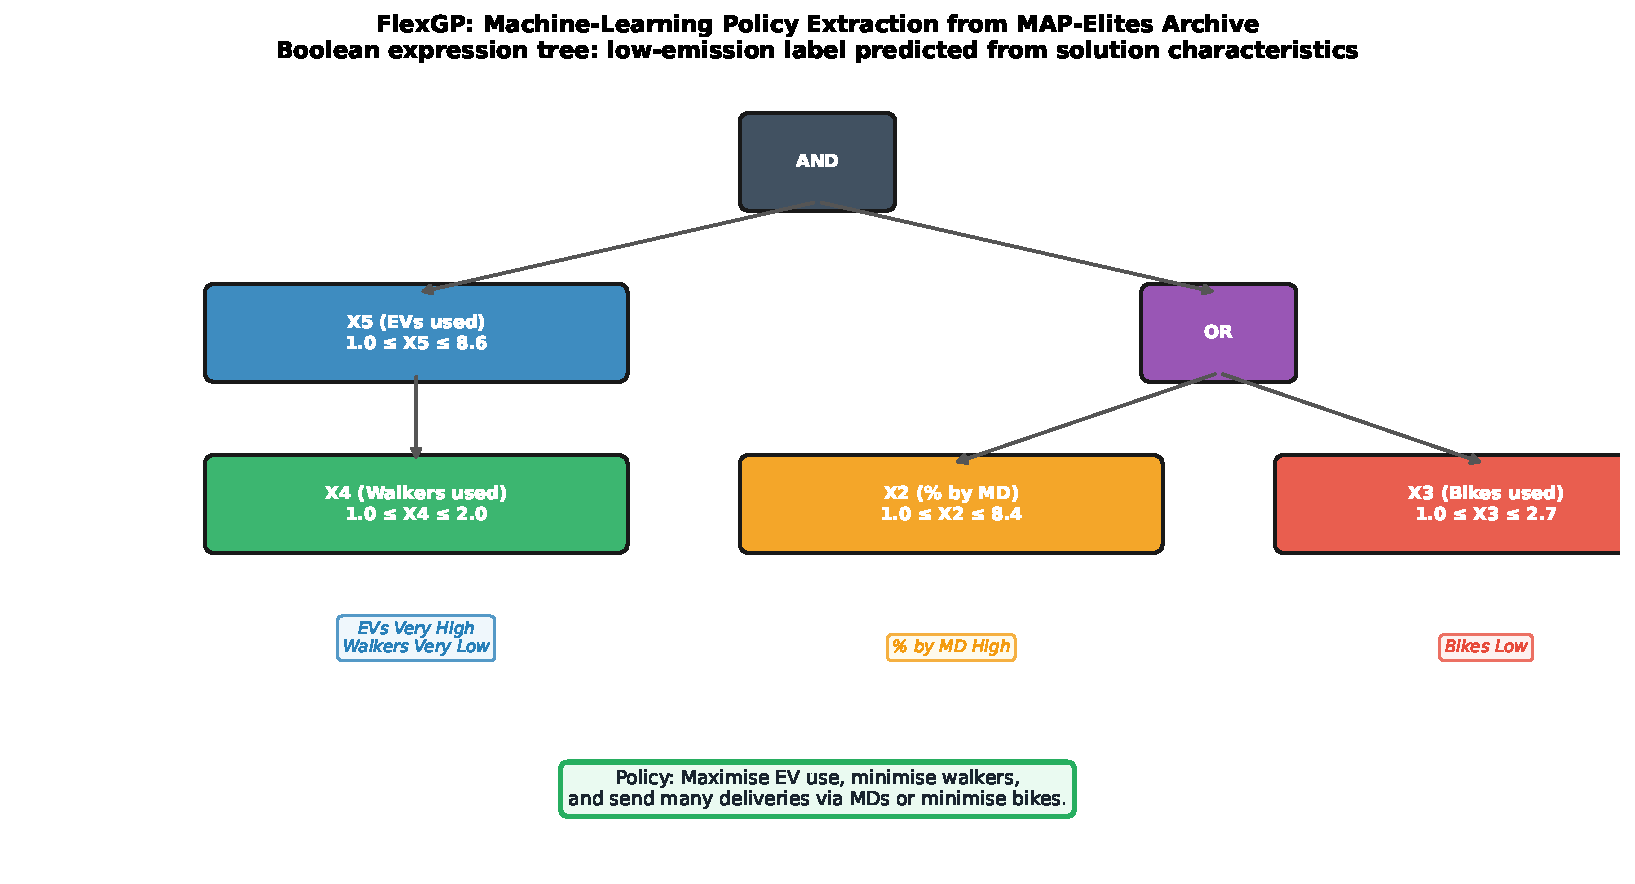
\includegraphics[width=0.85\textwidth]{fig_flexgp_policy}
\captionof*{figure}{\scriptsize The FlexGP Boolean decision tree for
  the low-emissions policy.
  Each leaf shows the translated natural-language label.}

\end{frame}

% ────────────────────────────────────────────────
\begin{frame}[allowframebreaks]{12.2 Why MAP-Elites Suits This Problem}

Several properties of the micro-depot delivery problem make MAP-Elites
a particularly good fit:

\medskip

\begin{enumerate}
  \item \textbf{Multiple objectives, multiple stakeholders.}
        A city authority cares about emissions; a courier company
        cares about delivery time; a resident cares about
        convenience.
        MAP-Elites maintains solutions optimised under all of these
        preferences simultaneously, rather than requiring the
        designer to specify weights upfront.

  \item \textbf{Heterogeneous operating conditions.}
        Some days have few deliveries; others are busy.
        Some neighbourhoods have cycle paths; others do not.
        MAP-Elites captures this variation because each archive
        cell corresponds to a different operating regime.

  \item \textbf{Decision support, not automation.}
        Logistics managers want to understand \emph{why} a policy
        works, not just execute a black-box recommendation.
        The FlexGP post-processing step converts the archive into
        transparent rules.

  \item \textbf{Computational scalability.}
        The archive representation allows MAP-Elites to scale
        to large problem instances without losing diversity,
        because solutions compete only within their own cell.
\end{enumerate}

\end{frame}

% ============================================================
\section{12.3 Implementation}
% ============================================================

\begin{frame}[allowframebreaks]{12.3 Software Architecture}

The implementation is built around a set of Python/Java classes.
The structure is shown in Figure~12.3 of the book.
The key design principle is \textbf{separation of concerns}:
the MAP-Elites search logic is kept separate from the logistics
simulation, which is itself kept separate from the results analysis.

\medskip

\begin{block}{Core Classes}
  \begin{tabular}{ll}
    \toprule
    \textbf{Class} & \textbf{Responsibility} \\
    \midrule
    \texttt{MDProblem}       & Encapsulates deliveries, MDs, couriers;
                               provides \texttt{solve()} and \texttt{evaluate()} \\
    \texttt{Model}           & Converts a chromosome into a delivery plan
                               (simulates the logistics network) \\
    \texttt{Results}         & Stores and exposes the solution:
                               cost, emissions, time, characteristics \\
    \texttt{MAPElites}       & Runs the archive-based evolutionary search \\
    \texttt{KeyGen}          & Computes the 7-dimensional archive key
                               from a \texttt{Results} object \\
    \texttt{Chromosome}      & Holds a variable-length list of \texttt{Gene} objects \\
    \texttt{Gene}            & One courier assignment:
                               (courier type, micro-depot ID, delivery quantity) \\
    \texttt{MicroDepot}      & Location and capacity of one micro-depot \\
    \texttt{Courier}         & Type, speed, capacity of one courier \\
    \bottomrule
  \end{tabular}
\end{block}

\medskip

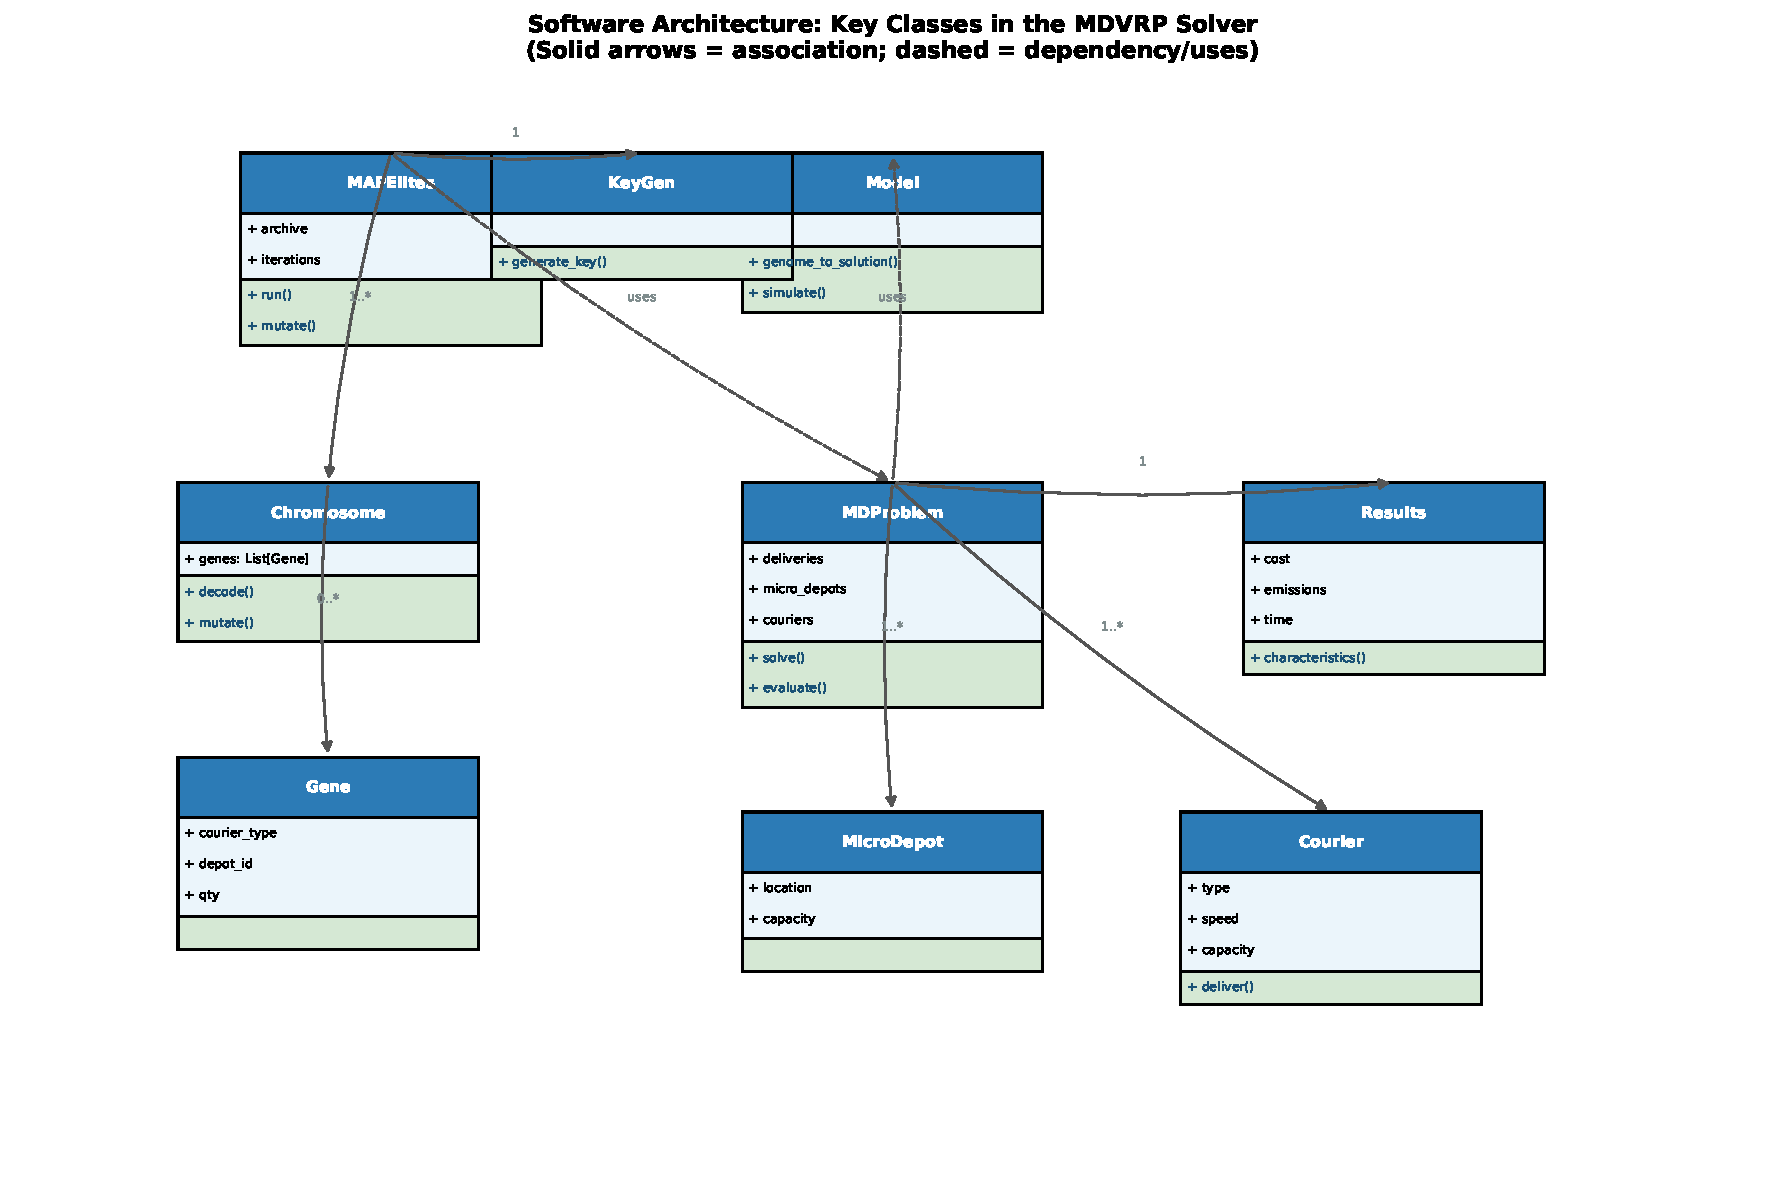
\includegraphics[width=0.88\textwidth]{fig_uml_class_diagram}
\captionof*{figure}{\scriptsize Stylised UML diagram of the main classes.
  Solid arrows = association; dashed = dependency.}

\end{frame}

% ────────────────────────────────────────────────
\begin{frame}[allowframebreaks]{12.3 Representation: Chromosomes and Genes}

The evolutionary algorithm works with \textbf{chromosomes},
which are the data structures it evolves.
Each chromosome represents one complete delivery plan.

\medskip

\begin{block}{Chromosome Structure}
  A chromosome is a variable-length ordered list of \textbf{genes}.
  Each gene encodes one courier assignment and contains exactly
  three pieces of information:
  \begin{enumerate}
    \item \textbf{Courier type}: one of \{walking, cycling, electric van\}.
    \item \textbf{Micro-depot ID}: which micro-depot this courier
          operates from.
    \item \textbf{Delivery quantity}: how many deliveries are
          transferred to this courier (an integer from 1 upward).
  \end{enumerate}
\end{block}

\medskip

\begin{exampleblock}{Example Gene}
  \begin{tabular}{lll}
    \toprule
    Courier type & Micro-depot & Quantity \\
    \midrule
    walking & MD2 & 3 \\
    \bottomrule
  \end{tabular}

  \smallskip
  This gene says: ``create a walking courier based at micro-depot~2,
  and assign it 3 deliveries from the default supply route.''
\end{exampleblock}

\medskip

\begin{exampleblock}{Example Chromosome (4 genes)}
  \begin{tabular}{llll}
    \toprule
    Gene & Courier type & Micro-depot & Quantity \\
    \midrule
    1 & walking       & MD2 & 3 \\
    2 & cycling       & MD1 & 4 \\
    3 & electric van  & MD3 & 4 \\
    4 & walking       & MD1 & 3 \\
    \bottomrule
  \end{tabular}

  \smallskip
  This chromosome describes a plan that uses four couriers
  across three micro-depots (MD1, MD2, MD3) to handle
  a total of $3+4+4+3 = 14$ deliveries.
\end{exampleblock}

\medskip

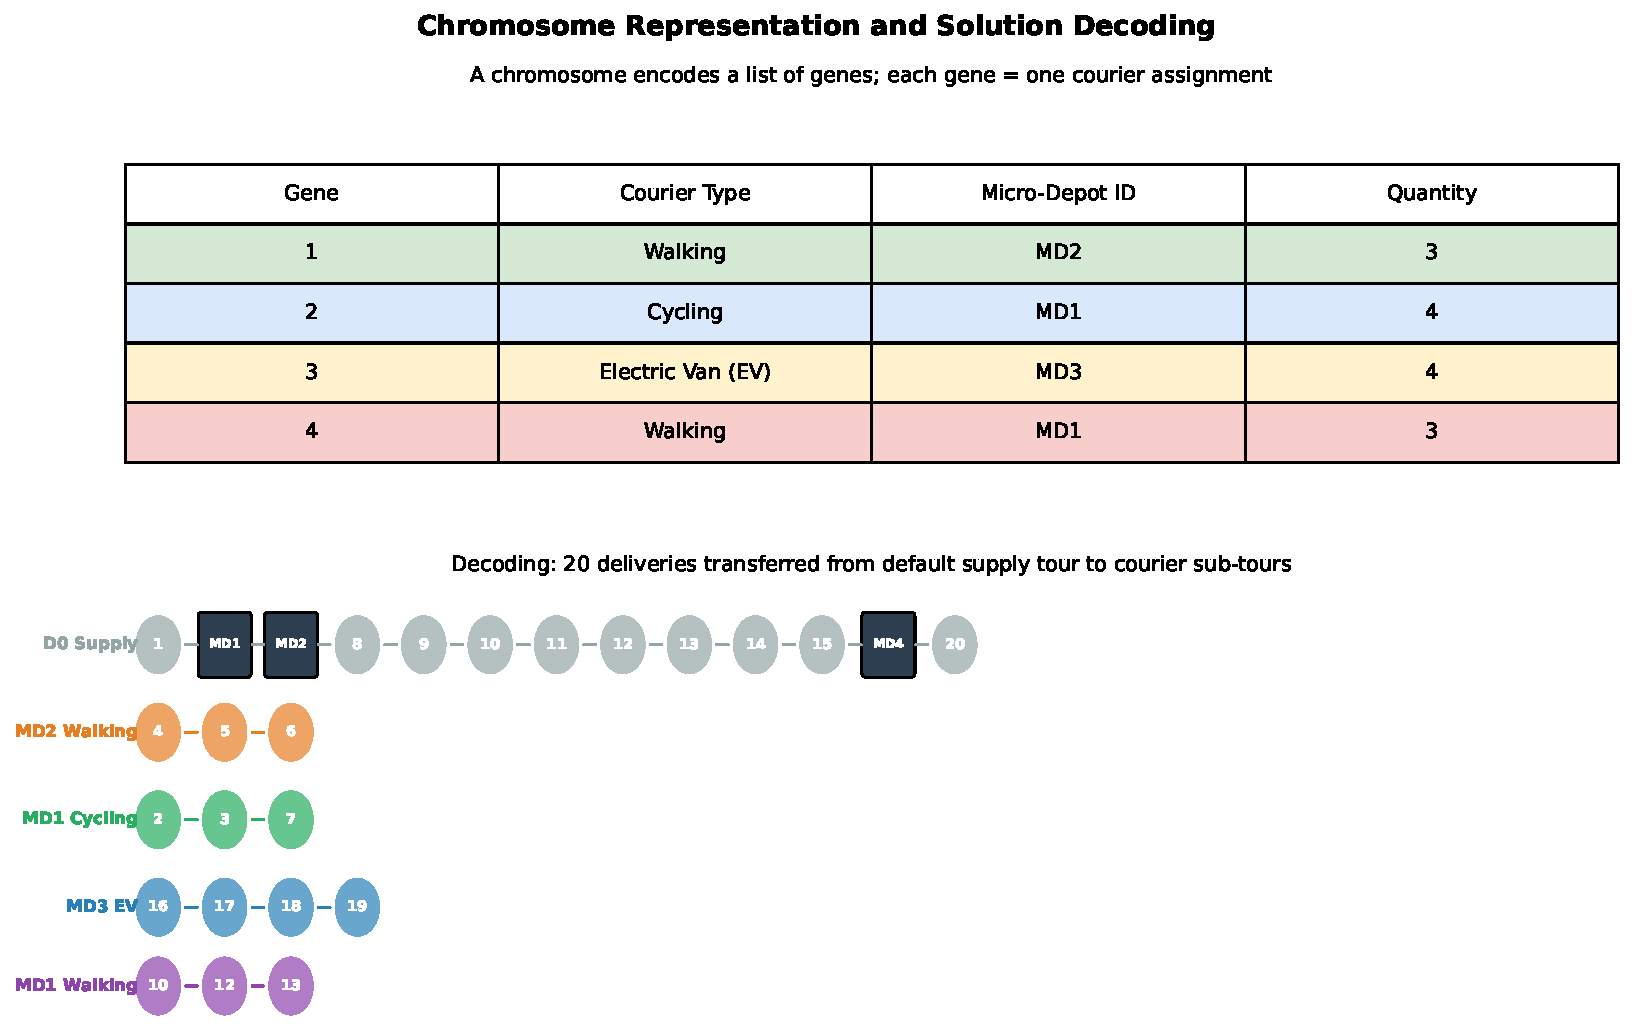
\includegraphics[width=0.95\textwidth]{fig_chromosome_decoding}
\captionof*{figure}{\scriptsize Top: gene table for a 4-gene chromosome.
  Bottom: the decoded delivery routes, showing how deliveries
  are transferred from the default supply tour.}

\end{frame}

% ────────────────────────────────────────────────
\begin{frame}[allowframebreaks]{12.3 Default Tour and the Nearest Neighbour Heuristic}

Every chromosome is decoded \emph{relative to} a \textbf{default tour}.
Understanding the default tour is essential for understanding
how the chromosome decoding works.

\medskip

\begin{block}{Default Tour}
  The default tour is the delivery plan that uses \emph{no} micro-depots
  and \emph{no} couriers: a single supply vehicle departs from the
  main depot D0 and visits all delivery addresses directly,
  in the order determined by the nearest-neighbour (NN) heuristic.

  The NN heuristic is a simple greedy construction method:
  starting from the depot, always travel next to the closest
  unvisited delivery point; repeat until all deliveries are served;
  then return to the depot.
  Although not optimal, NN is fast and produces a reasonable
  initial tour.
\end{block}

\medskip

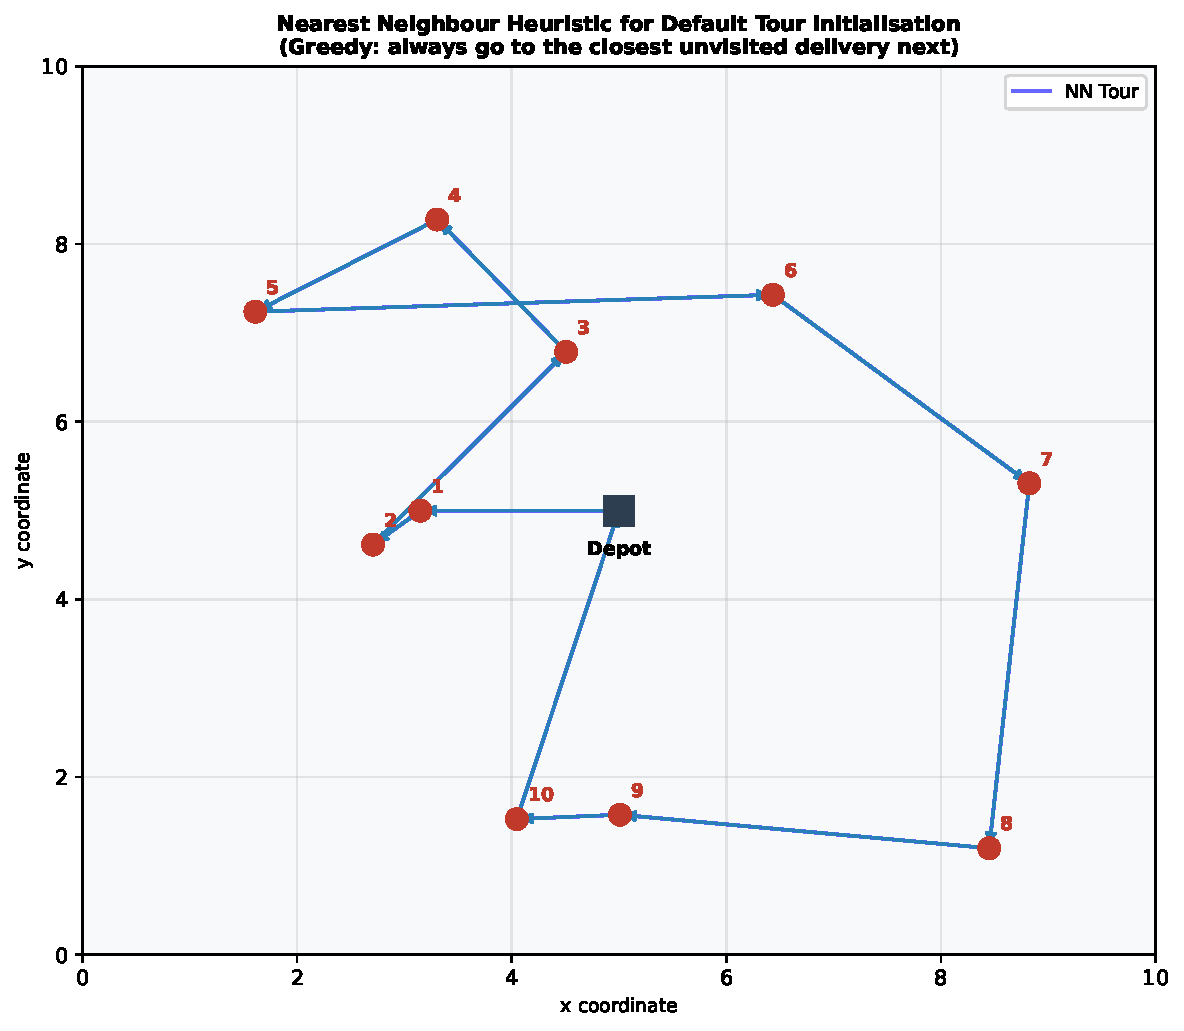
\includegraphics[width=0.55\textwidth]{fig_nearest_neighbour}
\captionof*{figure}{\scriptsize The nearest-neighbour heuristic builds
  the default tour greedily.
  Numbers show the visit order; the supply vehicle starts and ends
  at the depot (square).}

\medskip

The NN tour serves two purposes:
(1) it is the starting point that each chromosome tries to improve upon,
and (2) it is the fallback for any deliveries not assigned to a courier ---
the supply vehicle still handles them directly.

\end{frame}

% ────────────────────────────────────────────────
\begin{frame}[allowframebreaks]{12.3 Decoding a Chromosome --- Step by Step}

Decoding a chromosome means converting it from a list of genes
into a concrete delivery schedule with specific routes.
The decoding procedure follows Algorithm~24 (shown below)
for each gene in sequence.

\medskip

\begin{block}{Algorithm 24: Create Courier Tour}
  \textbf{Procedure} \texttt{createCourierTour(supplyTour, c, md, len)}

  \smallskip
  \begin{tabular}{ll}
    \textbf{Input} & \texttt{supplyTour}: the current supply vehicle tour \\
                   & \texttt{c}: courier type (walking/cycling/EV) \\
                   & \texttt{md}: the micro-depot this courier starts from \\
                   & \texttt{len}: the number of deliveries to transfer \\
    \textbf{Output} & A new courier sub-tour; \texttt{supplyTour} updated \\
  \end{tabular}

  \smallskip
  \begin{enumerate}
    \item Create an empty tour for courier $c$, starting at micro-depot \texttt{md}.
    \item Set \texttt{current} $\leftarrow$ \texttt{md}.
          Set \texttt{count} $\leftarrow 0$.
    \item \textbf{While} \texttt{count} $<$ \texttt{len}:
      \begin{enumerate}
        \item Find \texttt{del} = the delivery in \texttt{supplyTour} closest
              to \texttt{current} (using distances appropriate for vehicle type $c$).
        \item If the courier tour can still accommodate \texttt{del}
              (capacity not exceeded):
              add \texttt{del} to courier tour; remove from \texttt{supplyTour}.
              Increment \texttt{count}.
        \item Advance \texttt{current} $\leftarrow$ location of \texttt{del}.
      \end{enumerate}
    \item Find the insertion point in \texttt{supplyTour} closest to \texttt{md};
          insert a visit to \texttt{md} at that position
          (so the supply vehicle will deliver a batch to MD).
  \end{enumerate}
\end{block}

\medskip

The key function \texttt{findClosest(tour, loc, v)} searches the supply
tour for the stop closest to location \texttt{loc}, using distances
based on vehicle type \texttt{v} (walkers and cyclists can use paths
unavailable to larger vehicles, so their effective distance matrix differs).

\end{frame}

% ────────────────────────────────────────────────
\begin{frame}[allowframebreaks]{12.3 Worked Decoding Example --- 20 Deliveries}

Let us trace through decoding the example chromosome from page~244--245
of the book.
We have 20 deliveries, labelled 1--20.

\medskip

\textbf{Step~1: Initial default tour} (before decoding any genes).
All 20 deliveries are assigned to the supply vehicle at D0.

\begin{center}
  \begin{tabular}{lll}
    \toprule
    Depot & Vehicle/Courier & Deliveries \\
    \midrule
    D0 & Supply & 1 2 3 4 5 6 7 8 9 10 11 12 13 14 15 16 17 18 19 20 \\
    \bottomrule
  \end{tabular}
\end{center}

\medskip

\textbf{Step~2: Decode gene~1} (walking, MD2, qty~3).
The algorithm finds the 3 deliveries closest to MD2 in the supply tour
(starting from insertion position~4 in the NN order).
Customers 4, 5, 6 are extracted from the supply tour.
The supply tour now includes a stop at MD2 to drop off these parcels.

\begin{center}
  \begin{tabular}{lll}
    \toprule
    Depot & Vehicle/Courier & Deliveries \\
    \midrule
    D0  & Supply  & 1 2 3 MD2 7 8 9 10 11 12 13 14 15 16 17 18 19 20 \\
    MD2 & Walking & 4 5 6 \\
    \bottomrule
  \end{tabular}
\end{center}

\textbf{Step~3: Decode gene~2} (cycling, MD1, qty~4).
Customers 2, 3, 7 are nearest to MD1, so they are extracted.
Note that customer~2 position in the supply tour now points to MD1
(the supply vehicle visits MD1 to drop off 2, 3, 7).

\begin{center}
  \begin{tabular}{lll}
    \toprule
    Depot & Vehicle/Courier & Deliveries \\
    \midrule
    D0  & Supply  & 1 MD1 MD2 8 9 10 11 12 13 14 15 16 17 18 19 20 \\
    MD2 & Walking & 4 5 6 \\
    MD1 & Cycling & 2 3 7 \\
    \bottomrule
  \end{tabular}
\end{center}

\textbf{Step~4: Decode genes~3 and~4} (EV from MD3 and walking from MD1).
Two more courier routes are created.
Note that MD1 already appears in the supply tour from Step~3,
so no second visit to MD1 is needed for the walking courier;
the supply vehicle delivers to MD1 in one combined stop.

\begin{center}
  \begin{tabular}{lll}
    \toprule
    Depot & Vehicle/Courier & Deliveries \\
    \midrule
    D0  & Supply  & 1 MD1 MD2 8 9 11 14 15 MD4 20 \\
    MD2 & Walking & 4 5 6 \\
    MD1 & Cycling & 2 3 7 \\
    MD4 & EV      & 16 17 18 19 \\
    MD1 & Walking & 10 12 13 \\
    \bottomrule
  \end{tabular}
\end{center}

\begin{alertblock}{Key Insight}
  The supply vehicle now visits only 4 micro-depot stops
  (MD1 once, MD2, MD4, and delivers remaining directly),
  eliminating 14 of the original 20 in-city stops.
  The four couriers handle 14 deliveries using zero-emission
  or low-emission vehicles.
\end{alertblock}

\end{frame}

% ────────────────────────────────────────────────
\begin{frame}[allowframebreaks]{12.3 Evolutionary Operators}

MAP-Elites needs operators to \emph{generate} new candidate chromosomes
from existing archive entries.
The chapter uses standard evolutionary operators adapted for
variable-length chromosome lists.

\medskip

\begin{block}{Initialisation}
  During initialisation, each new chromosome is created with a
  randomly chosen number of genes between 0 and 10.
  Each gene's values (courier type, depot ID, quantity) are
  set randomly.
  A chromosome with 0 genes represents the default tour
  (no couriers at all), which is always a valid, feasible solution.
\end{block}

\medskip

\begin{block}{Mutation Operations (one chosen at random per generation)}
  \begin{enumerate}
    \item \textbf{Add gene}: append a new gene with random values.
          This grows the chromosome, testing new courier assignments.
    \item \textbf{Move gene}: randomly select one gene and move it
          to a different position in the list.
          The decoding order can affect which deliveries are
          transferred first, so position matters.
    \item \textbf{Alter gene}: randomly select one gene and randomly
          change one of its three values (type, depot, or quantity).
          This fine-tunes a specific courier assignment.
    \item \textbf{Delete gene}: randomly remove one gene.
          This reduces the number of couriers, testing whether
          a simpler plan performs as well.
  \end{enumerate}
\end{block}

\medskip

\begin{block}{Crossover}
  A new chromosome is created by selecting 10 genes from randomly
  chosen positions in a randomly selected parent chromosome.
  This produces offspring of length~10 that combine genes
  from different regions of the parent.
\end{block}

\medskip

\begin{alertblock}{Key Insight}
  Variable-length chromosomes allow the algorithm to automatically
  discover both the \emph{number} of couriers needed and their
  assignments.
  The designer does not need to specify how many couriers to use
  in advance --- the algorithm learns this from experience.
\end{alertblock}

\end{frame}

% ────────────────────────────────────────────────
\begin{frame}[fragile]{12.3 Python: MDProblem and Results Classes}

The following Python code sketches the core data structures
used in the implementation.
The \texttt{MDProblem} class holds all input data and
exposes a \texttt{solve()} method;
the \texttt{Results} class captures the output.

\begin{lstlisting}[caption={Core data structures (illustrative)}]
from dataclasses import dataclass, field
from typing import List
from enum import Enum

class CourierType(Enum):
    WALKING = "walking"
    CYCLING = "cycling"
    EV      = "electric_van"

@dataclass
class Gene:
    """One courier assignment: type, depot, quantity."""
    courier_type: CourierType
    depot_id: int       # which micro-depot (1-indexed)
    quantity: int       # number of deliveries to take

@dataclass
class Chromosome:
    """Variable-length list of genes (one gene = one courier)."""
    genes: List[Gene] = field(default_factory=list)

    def mutate_add(self, depot_ids, max_qty=10):
        import random
        self.genes.append(Gene(
            courier_type = random.choice(list(CourierType)),
            depot_id     = random.choice(depot_ids),
            quantity     = random.randint(1, max_qty)
        ))

    def mutate_delete(self):
        import random
        if self.genes:
            self.genes.pop(random.randrange(len(self.genes)))

    def mutate_alter(self, depot_ids, max_qty=10):
        import random
        if not self.genes:
            return
        g = random.choice(self.genes)
        field_idx = random.randint(0, 2)
        if field_idx == 0:
            g.courier_type = random.choice(list(CourierType))
        elif field_idx == 1:
            g.depot_id = random.choice(depot_ids)
        else:
            g.quantity = random.randint(1, max_qty)

@dataclass
class Results:
    """Stores computed solution metrics and characteristics."""
    total_cost: float = 0.0
    total_emissions: float = 0.0
    total_time: float = 0.0
    # The 7 characteristics normalised to scale 1-10
    n_mds_used: int = 1
    pct_by_md: int = 1
    bikes_used: int = 1
    walkers_used: int = 1
    evs_used: int = 1
    time_norm: int = 1
    emissions_norm: int = 1

    def characteristics(self):
        return (self.n_mds_used, self.pct_by_md, self.bikes_used,
                self.walkers_used, self.evs_used,
                self.time_norm, self.emissions_norm)
\end{lstlisting}

\end{frame}

% ────────────────────────────────────────────────
\begin{frame}[fragile]{12.3 Python: Nearest Neighbour Tour Construction}

The default tour is built by the nearest-neighbour heuristic.
The function below constructs this tour and returns the visit order.
This is the starting point for all chromosome decoding.

\begin{lstlisting}[caption={Nearest neighbour heuristic for default tour}]
import numpy as np

def nearest_neighbour_tour(depot, deliveries):
    """
    Build a nearest-neighbour tour starting and ending at the depot.

    Parameters
    ----------
    depot      : (float, float)  -- (x, y) coordinates of the main depot.
    deliveries : list of (float, float) -- customer locations.

    Returns
    -------
    tour_order : list of int -- indices into deliveries in visit order.
    """
    unvisited = list(range(len(deliveries)))
    tour_order = []
    current = np.array(depot)

    while unvisited:
        # Compute Euclidean distance from current location to all unvisited
        dists = [np.linalg.norm(np.array(deliveries[i]) - current)
                 for i in unvisited]
        nearest_idx = unvisited[int(np.argmin(dists))]
        tour_order.append(nearest_idx)
        current = np.array(deliveries[nearest_idx])
        unvisited.remove(nearest_idx)

    return tour_order

# Example: 5 deliveries in a small city area
depot = (0.0, 0.0)
customers = [(2.1, 3.5), (5.0, 1.2), (1.8, 7.0), (6.5, 4.4), (3.3, 6.1)]
order = nearest_neighbour_tour(depot, customers)
print("Default tour order:", order)
# => e.g. [0, 1, 3, 4, 2]  (greedy nearest-first)
\end{lstlisting}

\end{frame}

% ────────────────────────────────────────────────
\begin{frame}[fragile]{12.3 Python: Chromosome Decoding Loop}

The decoding loop iterates over the genes in a chromosome and
calls \texttt{create\_courier\_tour()} for each gene.
This progressively transfers deliveries from the supply tour
to courier sub-tours.

\begin{lstlisting}[caption={Chromosome decoding --- transfer deliveries to couriers}]
def decode_chromosome(chromosome, supply_tour, depots, couriers):
    """
    Decode a chromosome into a set of courier routes.

    Parameters
    ----------
    chromosome  : Chromosome object (list of genes)
    supply_tour : list of delivery indices (mutable -- will be modified)
    depots      : dict  {depot_id: (x, y)}  location of each micro-depot
    couriers    : list to accumulate (courier_type, depot_id, [deliveries])

    Returns
    -------
    couriers : list of (courier_type, depot_id, delivery_list)
    supply_tour : remaining deliveries for supply vehicle
    """
    for gene in chromosome.genes:
        ctype   = gene.courier_type
        md_id   = gene.depot_id
        qty     = gene.quantity
        md_loc  = depots.get(md_id)

        if md_loc is None:
            continue   # skip invalid depot reference

        courier_deliveries = []
        transferred = 0

        # Transfer up to qty deliveries closest to the micro-depot
        while transferred < qty and supply_tour:
            # Find closest delivery to current position of this courier
            current_pos = md_loc if not courier_deliveries else \
                          supply_tour[courier_deliveries[-1]]
            closest = min(supply_tour,
                          key=lambda d: distance(current_pos, d, ctype))
            courier_deliveries.append(closest)
            supply_tour.remove(closest)
            transferred += 1

        couriers.append((ctype, md_id, courier_deliveries))
        # Insert MD visit into supply tour at cheapest insertion point
        supply_tour.insert(find_insertion_point(supply_tour, md_loc), md_id)

    return couriers, supply_tour
\end{lstlisting}

\end{frame}

% ────────────────────────────────────────────────
\begin{frame}[fragile]{12.3 Python: MAP-Elites Archive and Main Loop}

The MAP-Elites archive is a dictionary mapping
a 7-tuple of integers (the characteristic key) to the best
\texttt{Results} object found for that key.

\begin{lstlisting}[caption={MAP-Elites archive and search loop}]
import random

def map_elites_run(problem, n_iterations=10000, init_pop=500):
    """
    Run MAP-Elites to fill the 7-D archive.

    Parameters
    ----------
    problem       : MDProblem instance
    n_iterations  : int -- number of MAP-Elites iterations
    init_pop      : int -- initial random population size

    Returns
    -------
    archive : dict  {(c1,...,c7): Results}
    """
    archive = {}   # key = 7-tuple, value = (fitness, chromosome, results)

    def insert(chrom, results):
        key = results.characteristics()
        fitness = -results.total_emissions   # maximise = minimise emissions
        if key not in archive or fitness > archive[key][0]:
            archive[key] = (fitness, chrom, results)

    # Phase 1: Initialisation -- random chromosomes
    for _ in range(init_pop):
        chrom = random_chromosome(problem.depot_ids)
        results = problem.solve(chrom)
        insert(chrom, results)

    # Phase 2: Iterative improvement
    for iteration in range(n_iterations):
        # Select a random elite from the archive
        _, parent_chrom, _ = random.choice(list(archive.values()))

        # Mutate the parent to create a new candidate
        child = copy_chromosome(parent_chrom)
        mutate(child, problem.depot_ids)       # one random mutation op

        # Evaluate and attempt to insert
        results = problem.solve(child)
        insert(child, results)

        if iteration % 1000 == 0:
            print(f"Iteration {iteration}: archive size = {len(archive)}")

    return archive
\end{lstlisting}

\end{frame}

% ────────────────────────────────────────────────
\begin{frame}[fragile]{12.3 Python: FlexGP Training Data Preparation}

After MAP-Elites produces the archive, we prepare training data
for FlexGP by labelling each solution based on its emissions level.

\begin{lstlisting}[caption={Prepare FlexGP training data from MAP-Elites archive}]
import csv

def prepare_flexgp_data(archive, emissions_threshold=3,
                        output_file="flexgp_data.csv"):
    """
    Convert the MAP-Elites archive into FlexGP training data.

    Label = 1 (very low emissions) if emissions_norm <= threshold,
    Label = 0 (higher emissions) otherwise.

    The 7 characteristics are: n_mds, pct_by_md, bikes, walkers,
    evs, time_norm, emissions_norm.
    The last column is the binary label.
    """
    rows = []
    for key, (fitness, chrom, results) in archive.items():
        c1, c2, c3, c4, c5, c6, c7 = results.characteristics()
        # Label: 1 = very low emissions (c7 <= threshold), 0 = otherwise
        label = 1 if c7 <= emissions_threshold else 0
        rows.append([c1, c2, c3, c4, c5, c6, label])

    with open(output_file, 'w', newline='') as f:
        writer = csv.writer(f)
        writer.writerow(['X1','X2','X3','X4','X5','X6','label'])
        writer.writerows(rows)

    print(f"Written {len(rows)} rows to {output_file}")
    print(f"Positive examples (low emission): {sum(r[-1] for r in rows)}")
    print(f"Negative examples: {len(rows) - sum(r[-1] for r in rows)}")

# Example call:
# prepare_flexgp_data(archive, emissions_threshold=3)
# Then run FlexGP externally:
# $ java -jar flexgp.jar --data flexgp_data.csv --output policy.txt
\end{lstlisting}

\end{frame}

% ============================================================
\section{12.4 Results}
% ============================================================

\begin{frame}[allowframebreaks]{12.4 Visualising the Archive: Parallel Coordinates}

After running MAP-Elites across the 10 problem instances,
the archives are \textbf{aggregated} to see patterns that hold
across different days and delivery loads.
The primary visualisation tool is the \textbf{parallel coordinates plot}.

\medskip

\begin{block}{What is a Parallel Coordinates Plot?}
  A parallel coordinates plot represents a high-dimensional solution
  as a single polyline drawn through a set of vertical axes.
  Each axis corresponds to one characteristic ($X_1$ through $X_7$).
  The position of the line on each axis shows the value of that
  characteristic for this particular solution.

  When many solutions are plotted together, the bundle of lines
  reveals structure: parallel bundles indicate correlation;
  crossing bundles indicate negative correlation (trade-offs).
\end{block}

\medskip


\includegraphics[width=\textwidth]{fig_parallel_coords}
\captionof*{figure}{\scriptsize Parallel coordinates of the MAP-Elites archive.
  Each line is one elite solution.
  Colour encodes total emissions level (green = low, red = high).
  Notice that low-emission lines (green) tend to have high values
  on the ``EVs Used'' axis and low values on ``Total Emissions''.}

\medskip

\begin{alertblock}{How to Read This Plot}
  Look for lines that cross between axes --- these indicate a trade-off
  (when one characteristic is high, the other tends to be low).
  For example, as ``EVs Used'' increases, the ``Emissions'' axis
  tends to decrease: the lines cross, showing a negative correlation.
  This is expected --- electric vehicles produce fewer emissions per delivery.
\end{alertblock}

\end{frame}

% ────────────────────────────────────────────────
\begin{frame}[allowframebreaks]{12.4 Heatmaps of Archive Coverage}

In addition to the parallel coordinates plot, the ElVis tool
(Urquhart, Neil, 2019) generates \textbf{heatmaps} for each
pair of solution characteristics.
A heatmap shows how densely populated each region of the
two-dimensional projection of the archive is, and how good
the solutions found there are.

\medskip

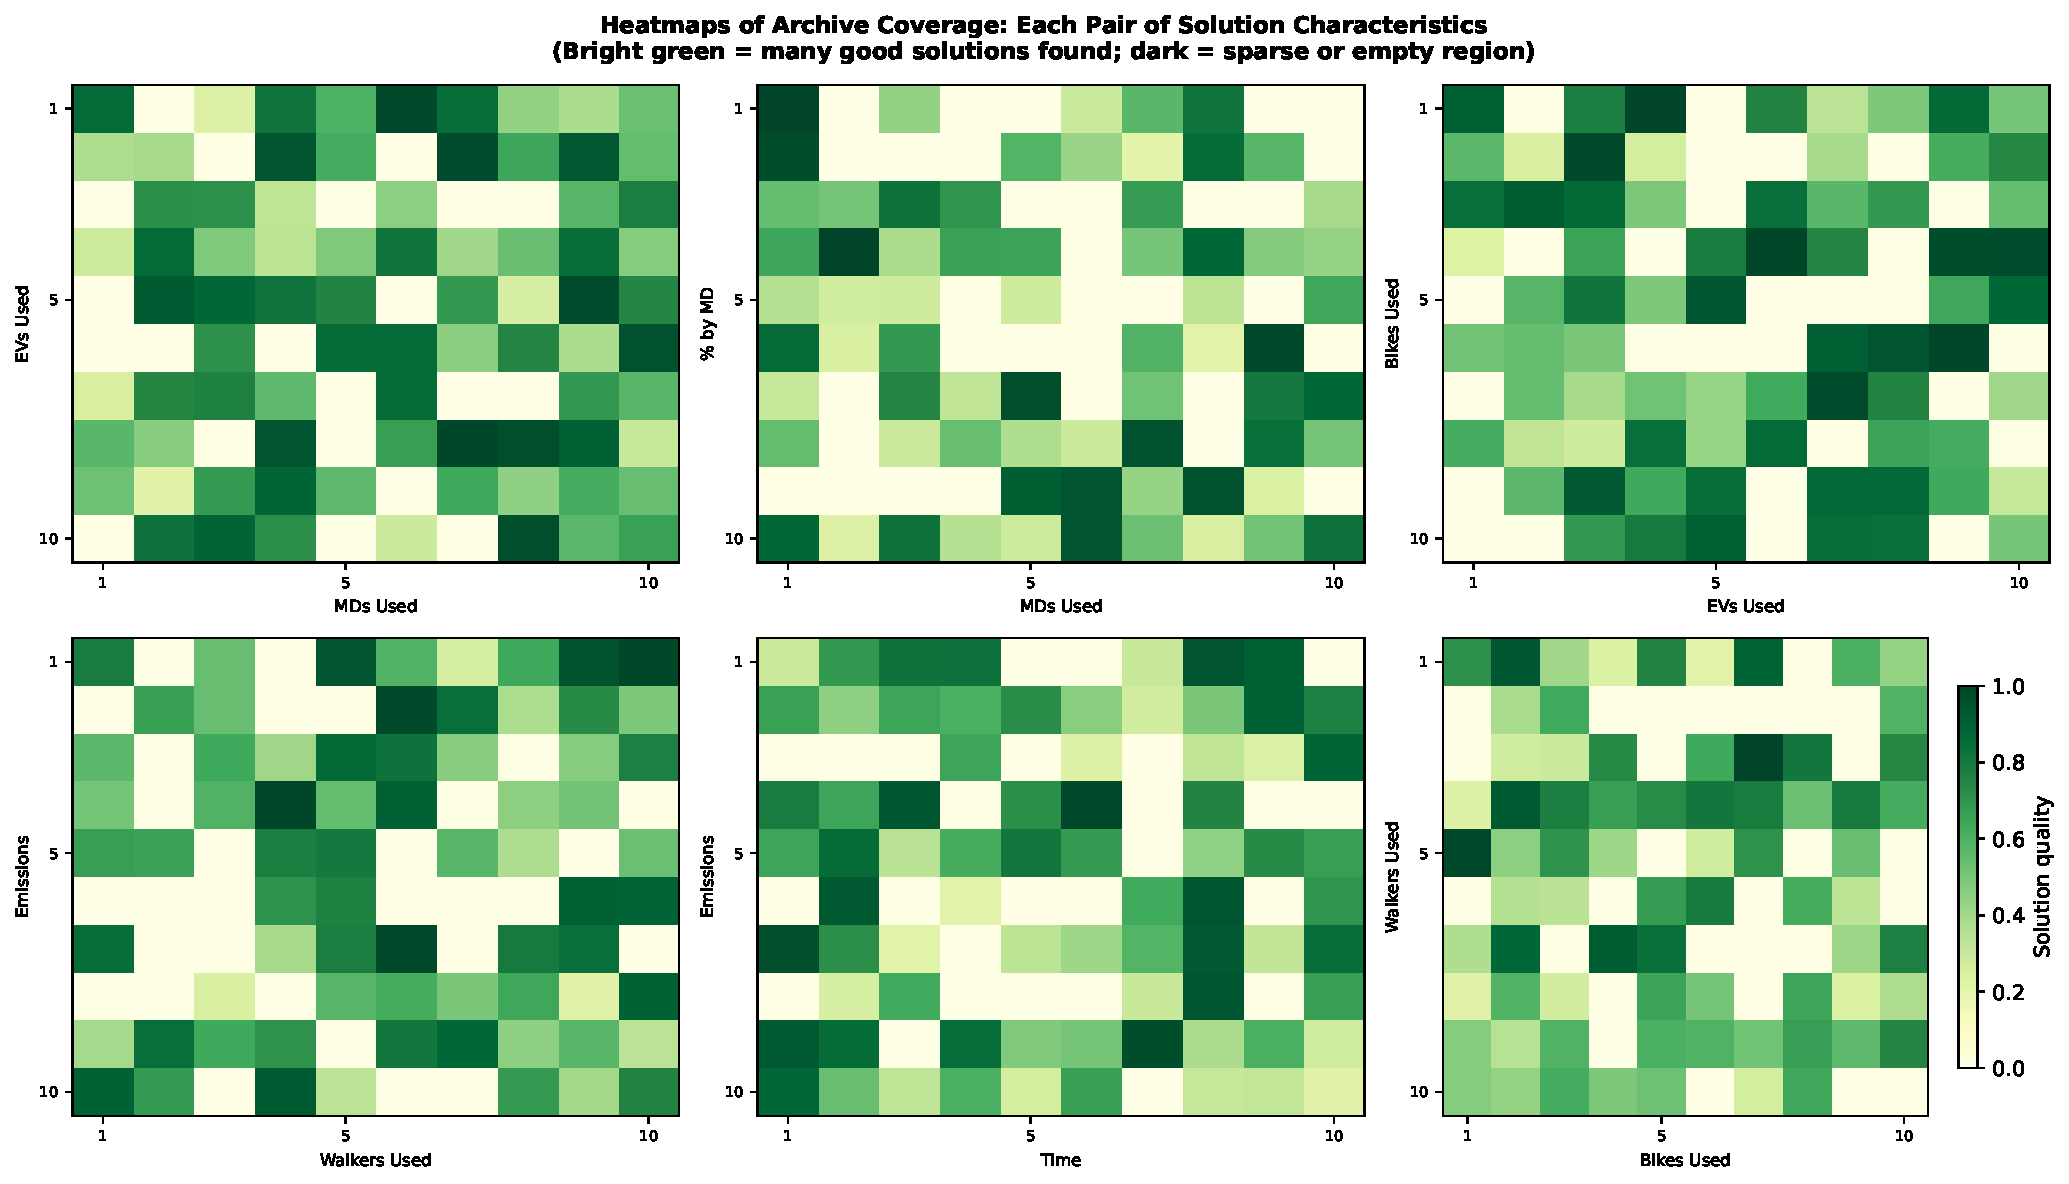
\includegraphics[width=0.92\textwidth]{fig_heatmap_pairs}
\captionof*{figure}{\scriptsize Heatmaps of archive coverage for six pairs
  of characteristics.
  Bright green cells contain high-quality solutions;
  dark cells are sparsely filled or empty.
  Gaps indicate regions of the solution space that the algorithm
  found difficult to populate --- either infeasible, or rarely visited.}

\medskip

\begin{block}{Interpreting Heatmap Gaps}
  It would be naive to assume that gaps in the heatmap represent
  \emph{impossible} solutions.
  More likely, the algorithm simply ran out of time to find good
  solutions in those regions.
  A gap is an invitation to investigate: could a targeted search
  in that region yield useful solutions?
\end{block}

\medskip

The heatmaps are particularly useful for comparing archives
across different problem instances (different days).
If a gap appears consistently across all 10 instances,
it provides stronger evidence that the region is genuinely
hard to populate.

\end{frame}

% ────────────────────────────────────────────────
\begin{frame}[allowframebreaks]{12.4 Which Factors Lead to Reduced Delivery Time?}

The first policy question the chapter investigates is:
\textbf{which factors in a solution lead to shorter delivery times?}

\medskip

To answer this, the archive is filtered to identify solutions
with low values on the ``Total Time'' characteristic ($X_6$).
FlexGP is run on this filtered dataset.
The resulting raw policy (based on the knee of the Pareto front
for time) is:

\begin{block}{FlexGP Policy: Fast Delivery}
  \[
    E1 \le X1 \le E2 \quad \text{and} \quad 3 \le X5 \le 10.16
  \]
  where $X1$ = number of micro-depots used and $X5$ = EVs used.
  After substituting labels: $E1, E2$ refer to specific range boundaries.
  An example interpretation from the book (p.~248):
  \[
    1.0 \le X1 \le 3 \quad \Rightarrow \quad \text{MicroDepotsUsed} \le \text{Low}
  \]
\end{block}

\medskip

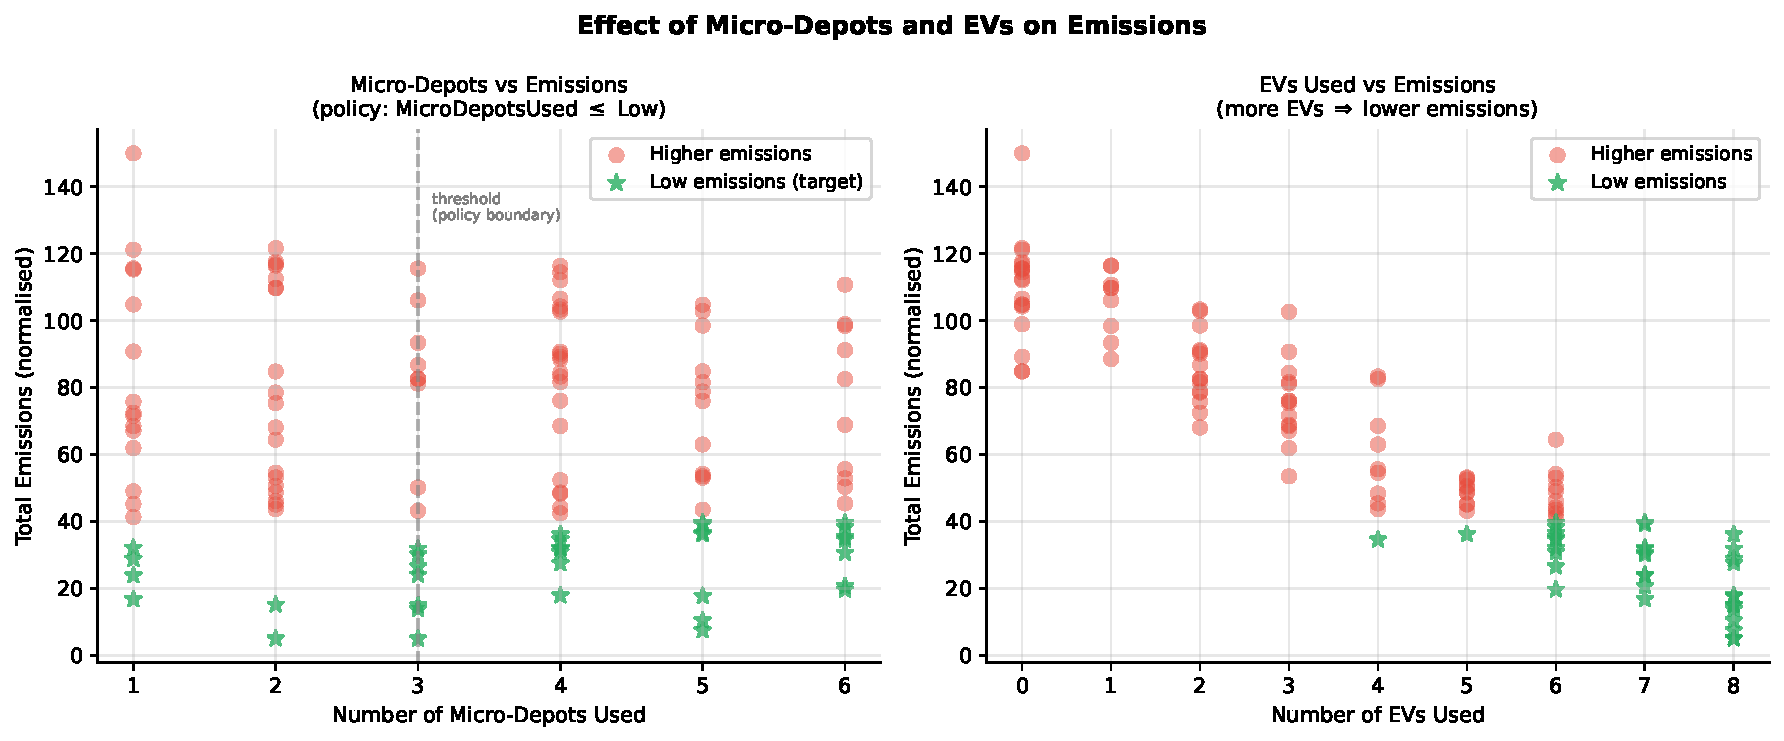
\includegraphics[width=0.92\textwidth]{fig_low_emissions}
\captionof*{figure}{\scriptsize Left: number of micro-depots vs.\ emissions
  (stars = low-emission solutions; policy boundary shown dashed).
  Right: EVs used vs.\ emissions (more EVs strongly reduces emissions).}

\medskip

\begin{alertblock}{Key Insight from the Time Analysis}
  The analysis reveals that having \emph{few} micro-depots and using
  EVs (fast couriers) leads to faster overall delivery.
  This is counterintuitive at first glance --- one might expect
  more micro-depots to speed things up.
  But the overhead of visiting and stocking many micro-depots
  slows the supply vehicle down, negating the benefit of faster
  last-mile couriers.
  The sweet spot is to use a small number (1--3) of well-placed
  micro-depots, each stocked efficiently by the supply vehicle.
\end{alertblock}

\end{frame}

% ────────────────────────────────────────────────
\begin{frame}[allowframebreaks]{12.4 Which Factors Lead to Low Emissions?}

The second policy question is:
\textbf{which combinations of solution characteristics lead to
low total emissions?}

\medskip

\begin{block}{FlexGP Raw Policy (Low Emissions)}
  \[
    \bigl((1.0 \le X_5 \le 8.6\ \mathbf{and}\ 1.0 \le X_4 \le 2.0)\
    \mathbf{and}\ (1.0 \le X_2 \le 8.4\ \mathbf{or}\ 1.0 \le X_3 \le 2.7)\bigr)
  \]
  After substituting labels:
  \[
    ((\text{EVsUsed} \le \text{VeryHigh}\
    \mathbf{and}\ \text{WalkersUsed} \le \text{VeryLow})\
    \mathbf{and}\
    (\%\text{ByMD} \le \text{High}\ \mathbf{or}\ \text{BikesUsed} \le \text{Low}))
  \]
\end{block}

\medskip

The plain-English interpretation of this policy is:
\begin{quote}
  \emph{Maximise the use of EVs and make minimum use of walking couriers.
  And send as many deliveries via micro-depots as possible,
  or minimise the use of bicycles.}
\end{quote}

\medskip

This policy makes sense for the following reasons:

\begin{itemize}
  \item Walking couriers complete very few deliveries per hour
        compared to EVs. Using many walkers means the supply vehicle
        must make many small deliveries to many micro-depots,
        which itself adds emissions.
  \item EVs are the fastest and highest-capacity green couriers.
        Fewer total trips are needed when EVs are used.
  \item Maximising the fraction of deliveries through MDs
        (\%ByMD is High) ensures that the supply vehicle
        makes efficient batch transfers rather than many small city trips.
\end{itemize}

\end{frame}

% ────────────────────────────────────────────────
\begin{frame}[allowframebreaks]{12.4 Can We Achieve Low Emissions AND Fast Delivery Together?}

A natural follow-up question is whether low emissions and fast delivery
can be achieved \emph{simultaneously}, or whether they are always in conflict.

\medskip

\begin{block}{FlexGP Analysis: Combined Objective}
  Solutions that achieve both low emissions and fast delivery time
  were highlighted.
  Running FlexGP on this combined subset yields the policy:
  \[
    1.0 \le X_1 \le 3 \quad \Rightarrow \quad \text{MicroDepotsUsed} \le \text{Low}
  \]
  That is, the distinguishing factor is simply the number of micro-depots:
  using \textbf{at most 3} micro-depots simultaneously achieves
  both low emissions and fast delivery.
\end{block}

\medskip

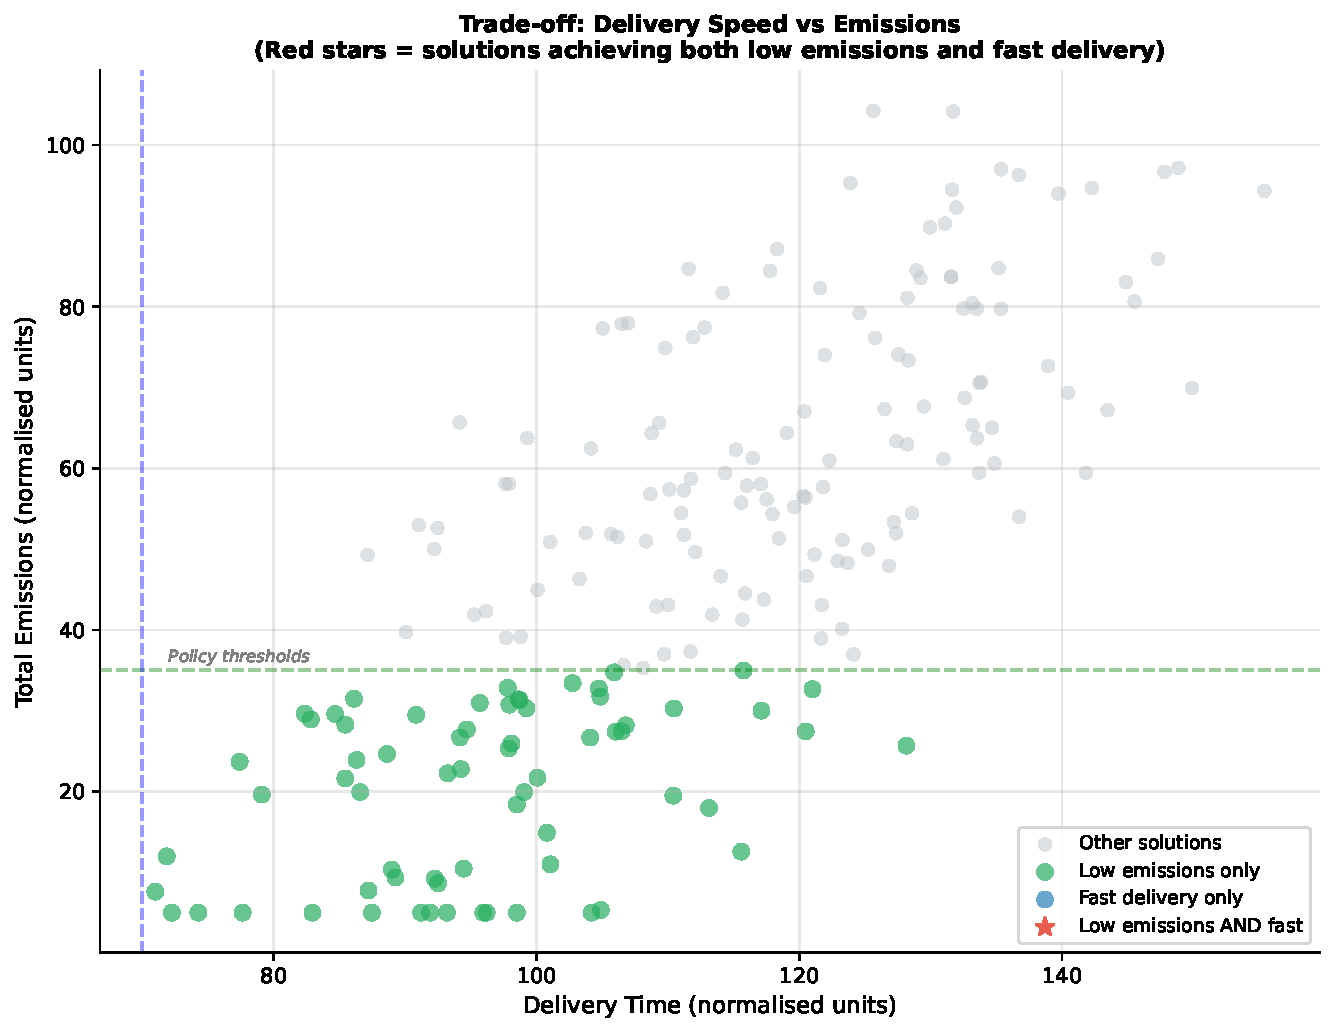
\includegraphics[width=0.85\textwidth]{fig_emissions_time_tradeoff}
\captionof*{figure}{\scriptsize Scatter plot of delivery time vs.\ emissions.
  Red stars = solutions that are both fast AND low-emission.
  These cluster in the lower-left corner and are characterised
  by few micro-depots (1--3) and high EV use.}

\medskip

\begin{alertblock}{Surprising Insight}
  The emission and time objectives are \emph{not} fundamentally in conflict.
  Both are minimised by using a small number of micro-depots and
  prioritising EVs.
  The reason is that the \emph{overhead} of managing many micro-depots
  --- the supply vehicle making multiple trips, couriers walking slowly ---
  harms both speed and emissions.
  A lean, EV-heavy, few-MD design wins on both dimensions.
\end{alertblock}

\end{frame}

% ────────────────────────────────────────────────
\begin{frame}[allowframebreaks]{12.4 Summary of Policy Findings}

The MAP-Elites + FlexGP pipeline produces the following
actionable insights for Edinburgh parcel delivery:

\medskip

\begin{block}{Policy Summary Table}
  \begin{tabular}{lll}
    \toprule
    \textbf{Objective} & \textbf{Key Factor(s)} & \textbf{Direction} \\
    \midrule
    Reduce emissions & EVs Used & Maximise \\
    Reduce emissions & Walkers Used & Minimise \\
    Reduce emissions & \% via Micro-Depots & Maximise \\
    Reduce emissions & Bikes Used & Minimise \\
    Reduce delivery time & Micro-Depots Used & Use few (1--3) \\
    Reduce delivery time & EVs Used & Maximise \\
    Both (combined) & Micro-Depots Used & $\le 3$ \\
    \bottomrule
  \end{tabular}
\end{block}

\medskip

These policies are \textbf{stable across 10 problem instances},
which provides confidence that they reflect genuine structural
properties of the Edinburgh city centre scenario
rather than artefacts of a single day's data.

\medskip

\begin{alertblock}{Operational Recommendation}
  A city logistics operator should: (1) deploy 1--3 micro-depots
  at strategic city-centre locations, (2) prioritise electric vans
  for courier assignments, and (3) use walking couriers only as a
  last resort (e.g.\ for addresses accessible only on foot).
  This strategy reduces both emissions and delivery time simultaneously.
\end{alertblock}

\end{frame}

% ============================================================
\section{12.5 Conclusions}
% ============================================================

\begin{frame}[allowframebreaks]{12.5 Conclusions}

This chapter has demonstrated a complete pipeline for
solving and understanding the urban parcel delivery problem
using nature-inspired optimisation.

\medskip

\begin{block}{Main Contributions}
  \begin{enumerate}
    \item \textbf{MAP-Elites as a decision-support tool}:
          rather than returning a single delivery plan,
          MAP-Elites returns an entire library --- one best plan
          for each combination of characteristics.
          Logistics planners can select the plan that best matches
          today's priorities (low cost, low emissions, fast delivery).

    \item \textbf{Variable-length chromosome representation}:
          the gene-based encoding allows the algorithm to automatically
          discover both the number of couriers and their assignments,
          without requiring the human to specify this in advance.
          Genes are added, removed, or altered by mutation operators.

    \item \textbf{FlexGP policy extraction}:
          machine learning converts the archive data into
          compact, human-readable Boolean rules.
          This closes the loop between optimisation and managerial
          decision-making --- a manager can act on the policy
          without understanding the underlying algorithm.

    \item \textbf{Stable policies across instances}:
          the finding that 1--3 micro-depots with high EV usage
          dominates both the emissions and time objectives is
          consistent across all 10 problem instances.
  \end{enumerate}
\end{block}

\medskip

\begin{block}{Limitations and Open Questions}
  \begin{itemize}
    \item The analysis uses relatively small problem instances
          (one day's deliveries in a city centre).
          Scaling to larger instances (hundreds of deliveries,
          many city districts) is an open challenge.
    \item The courier speed and capacity values are stylised.
          Real data (e.g.\ from GPS traces) would improve accuracy.
    \item FlexGP produces one policy per objective.
          A multi-objective FlexGP that produces Pareto-optimal
          policies simultaneously would be valuable.
    \item Dynamic re-planning (as new orders arrive through the day)
          is not addressed.
  \end{itemize}
\end{block}

\medskip

\begin{alertblock}{Closing Thought}
  The most important lesson from Chapter~12 is that
  the question ``What is the best delivery plan?'' is
  the wrong question for complex urban logistics.
  The right question is ``What is the best plan \emph{given
  today's priorities}, and what does the space of trade-offs
  look like?''
  MAP-Elites, combined with transparent policy extraction,
  answers the right question.
\end{alertblock}

\end{frame}

% ────────────────────────────────────────────────
\begin{frame}[allowframebreaks]{References}
  \begin{itemize}
    \item Mouret, J.-B. and Clune, J. (2015). Illuminating search spaces
          by mapping elites. \textit{arXiv:1504.04909}.
    \item Urquhart, N., H\"{o}hl, S. and Hart, E. (2019).
          An illumination algorithm approach to solving the micro-depot
          routing problem. \textit{Proceedings of GECCO 2019}, ACM,
          pp.~1347--1355.
    \item Urquhart, N., H\"{o}hl, S. and Hart, E. (2021).
          Automated, Explainable Rule Extraction from MAP-Elites Archives.
          \textit{EvoApplications 2021}, LNCS Vol.~12694, pp.~258--272.
    \item Group, A. (n.d.). Rule Tree Learner.
          \url{http://flexgp.github.io/gp-learners/ruletree.html}
    \item Urquhart, Neil (2019). ELite VISualisation (ElVis).
          \url{https://commute.napier.ac.uk/upload}
    \item Browne, M., Allen, J., and Leonardi, J. (2011).
          Evaluating the use of an urban consolidation centre and
          electric vehicles in central London.
          \textit{IATSS Research} 35(1):1--6.
    \item Fischer, M. (2017). \textit{City Logistics: Determination
          of Criteria to Evaluate Locations for Micro-Depots in
          Frankfurt am Main}. Master's thesis, Frankfurt University
          of Applied Science.
  \end{itemize}
\end{frame}

% ────────────────────────────────────────────────
\begin{frame}{End of Chapter 12}
  \begin{center}
    \Large\textbf{Chapter 12: Delivering Parcels}

    \bigskip
    \normalsize
    Key theme: MAP-Elites illuminates the solution space for
    urban parcel delivery via micro-depots and green couriers.
    FlexGP extracts actionable, human-readable policies.

    \bigskip
    \textbf{Core finding:} Use 1--3 micro-depots with electric vehicles
    to simultaneously minimise emissions and delivery time
    in the Edinburgh city-centre scenario.
  \end{center}
\end{frame}

\end{document}
